\RequirePackage{iftex}
\ifPDFTeX
\documentclass[a4paper,12pt]{article}
\usepackage[margin=24mm]{geometry}
\usepackage[T1]{fontenc}
\usepackage[utf8]{inputenc}
\usepackage{graphicx}
\usepackage{CJKutf8}
\else
\documentclass[a4paper,12pt]{jsarticle}
\usepackage[dvipdfmx,margin=24mm]{geometry}
\usepackage[dvipdfmx]{graphicx}
\fi
\usepackage{amsmath,amssymb,amsthm}
\usepackage{enumitem}
\usepackage{tikz}
\usetikzlibrary{arrows.meta}

\setlength{\parindent}{0pt}
\setlength{\parskip}{0.35em}
\setlist[itemize]{leftmargin=2em,itemsep=0.2em,topsep=0.3em}

\newcommand{\feedbackqa}[2]{%
\item[]
\begin{tabular}[t]{@{}p{1.8em}@{\hspace{0.4em}}p{\dimexpr\linewidth-2.2em\relax}@{}}
Q. & #1 \\
A. & #2
\end{tabular}
\par\smallskip\hrulefill
}

\newcommand{\feedbacknote}[1]{%
\item[] #1\par\smallskip\hrulefill
}

\newcommand{\feedbackrule}{%
\item[] \leavevmode\hrulefill
}

\begin{document}
\ifPDFTeX
\begin{CJK}{UTF8}{min}
\fi
\theoremstyle{definition}
\newtheorem*{definition}{定義}
\newtheorem*{theorem}{定理}

\begin{center}
{\LARGE 数学1A 第2回レジュメ}\\[0.4em]
連続と微分の基本
\end{center}
\section*{フィードバック}

\begin{itemize}[leftmargin=1.5em,itemsep=0.7em,topsep=0.3em]
\feedbackqa{太文字($\mathbb N,\mathbb R$など)の文字の書き方がわからない}{一本線を足すだけです。}
\feedbackqa{$x\in (0,\infty)$ と書くとき、実数であることを明確にするために、$x \in \mathbb{R}$ かつ $x\in (0,\infty)$ と書かなくてよいのか。}{もちろん $x\in \mathbb{R}$ かつ $x\in (0,\infty)$ と書いてもよいですが、通常は $x\in (0,\infty)$ とだけ書きます。理由は、$(0,\infty)$ は $\mathbb{R}$ の部分集合として定義されているので、$x\in (0,\infty)$ だけで実数だとわかるからです。（ちなみに複素数の場合は $x>0$ という順序が定義できないので、実数となります。）}
\feedbackqa{自分の記号の字が雑すぎて、バツにされないか不安}{回答を見る限り、普通に読めます。むしろ読みやすいくらいなので大丈夫です。}
\feedbackqa{理解するのが急に難しくなる分野はあるか}{数学でいうと、集合論や位相のあたりは急に難しく感じる人が多いです。}
\feedbackqa{眠い}{一限なので大変ですが、頑張りましょう。}
\feedbackqa{ワクワクする不定積分は何でしょう？（答えは $\int 1\,dx = x+C$、つまり「エックスたすシー」）}{……。}
\feedbackqa{教科書で勉強すれば期末を乗り切れるか}{教科書の範囲から出ますが、過去問を見た感じでは難易度はもう少し高いように思います。（同級生と対策セミナーのようなものを開いてみるとよいかもしれません。）}
\feedbackqa{再履がんばります}{ぜひ頑張りましょう。}
\feedbackqa{授業のノートを取るにあたり、手書きかタブレットか、どちらがよいか}{これは好みの問題ですが、私は手書きのほうが頭に入りやすい気がします。}
\feedbackqa{$\epsilon$-$\delta$ が、これでなぜ定義になっているのか知りたい}{実は、極限の定義の仕方は $\epsilon$-$\delta$ 以外にもいくつかあります。$\epsilon$-$\delta$ が採用されているのは、便利だからという理由が一番大きいと思います。直感的には、$<\delta$ や $<\epsilon$ は「十分小さい」という意味です。したがって、$|x-a|<\delta$ は「$x$ が $a$ に十分近い」、$|f(x)-b|<\epsilon$ は「$f(x)$ が $b$ に十分近い」ということなので、直感ともそれほど離れていない定義だと理解しています。}
\feedbackqa{高校の内容で復習したほうが良いものはあるか}{復習しておいたほうがよい高校範囲は、数学II・IIIの微積です。定義だけでも見ておくとよいと思います。}
\feedbackqa{もっと論理っぽいことをやりたい}{学科の枠を越えて、数理科学科でお待ちしています。}
\feedbackqa{オンデマンドをやる予定はあるか？}{6月の第2週に出張が入っているので、そのときはオンデマンドになると思います。}
\feedbackqa{暗記より理解するほうが大事か？}{どちらも大事だと思います。暗記しているうちに、自然に考えが深まって理解につながることもあります。（自分は $\epsilon$-$\delta$ の理解がそんな感じでした。）}
\feedbackqa{ギリシャ文字を書くのが苦手}{ぜひ周りの人に確認してもらいましょう。}
\feedbackqa{$\epsilon$-$\delta$ をやる理由}{使っているとわかりますが、説明するときに便利だというのが自分の認識です。}
\feedbackqa{演習問題を載せたプリントを配布してほしい。}{レポートを2回配る予定です。それ以外は教科書の演習問題を解いてほしいと思います（解答は巻末についています）。}
\feedbackqa{教科書の使い方について}{授業でわからなかったところや、授業で扱わなかったところを復習するのに使うとよいと思います。}
\feedbackqa{Word で数式をどうやって入力する？}{私は Word で数式入力をすることがないので、あまりよくわかりません。（たしか「数式」というタブがあったような気もします。）基本的には LaTeX という枠組みを使うことが多いです。}
\feedbackqa{$0<x$ と書いたとき、虚数はなぜ含まれないか？}{虚数には順序がないので、$0<x$ と書いた瞬間に $x$ は実数となります。}
\feedbackqa{おすすめの問題集}{指定した教科書くらいしか知らないですね。}
\feedbackqa{欠席した場合はどう勉強すればよいか？}{教科書を読んでいただいて、わからないところがあれば聞いてください。}
\feedbackqa{予習の仕方}{授業が始まる前に数分でもよいので、教科書に出てくる単語を眺めておくのはしたほうがよいと思います。可能であれば、ある程度理解したうえで授業に臨むのがベストです。}
\feedbackqa{$\epsilon$-$\delta$ 論法をやっていると、理解していないのにできている気分になる。}{とりあえずはそれでよいと思いますし、ルールどおりにできることが理解の第一歩だと思います。}
\feedbackqa{なぜ $|x-a|<\delta$ には $\delta$ を、$|f(x)-b|<\epsilon$ には $\epsilon$ を使うのか？}{よい質問ですね。これは単純に慣習的なもので、特に深い意味はありません。逆に「任意の $\delta$ について、ある $\epsilon$ が存在して、$|x-a|<\epsilon$、$|f(x)-b|<\delta$」と書いても、まったく問題ありません。}
\end{itemize}

\section*{小テスト}

\subsection*{問題}

問1. 次を言い換えよ。
\begin{itemize}
\item $(1)$ $a$ を実数とする
\item $(2)$ $x$ を負の実数とする
\end{itemize}

問2. $\epsilon$-$\delta$ 論法で
\[
\lim_{x\to 1}(x-2)=-1
\]
を示せ。

\subsection*{解答}

問1.
\begin{itemize}
\item $(1)$ $a\in \mathbb{R}$
\item $(2)$ $x\in (-\infty,0)$
\end{itemize}

問2.

任意の $\epsilon>0$ をとる。ここで
\[
\delta=\epsilon
\]
とおく。$|x-1|<\delta$ ならば
\[
|(x-2)-(-1)|=|x-1|<\delta=\epsilon
\]
である。したがって
\[
\lim_{x\to 1}(x-2)=-1
\]
が成り立つ。

\section*{1. 連続の定義}

\begin{definition}
関数 $f$ が点 $a$ で連続であるとは，
\[
\lim_{x \to a} f(x)=f(a)
\]
が成り立つことをいう。
\end{definition}

$f$ が区間 $I$ で連続であるとは，$I$ の各点で連続であることをいう。

\section*{2. 連続の例}

\subsection*{例1. $f(x)=x$}

$f(x)=x$ は $\mathbb{R}$ で連続。

\begin{center}
\begin{tikzpicture}[x=1cm,y=1cm]
\draw[->] (-2.3,0) -- (2.3,0) node[below] {$x$};
\draw[->] (0,-2.3) -- (0,2.3) node[left] {$y$};
\draw[thick,domain=-2:2,samples=2] plot (\x,\x);
\draw (1.6,1.9) node[right] {$f(x)=x$};
\end{tikzpicture}
\end{center}

\subsection*{例2. $f(x)=\mathbf{1}_{\{x\ge 0\}}$}

\[
f(x)=
\begin{cases}
0 & (x<0),\\
1 & (x\ge 0)
\end{cases}
\]
とする。$x=0$ で不連続。
\[
\lim_{x\to 0-}f(x)=0,\qquad \lim_{x\to 0+}f(x)=1
\]

\begin{center}
\begin{tikzpicture}[x=1.4cm,y=1.4cm]
\draw[->] (-2.2,0) -- (2.2,0) node[below] {$x$};
\draw[->] (0,-0.4) -- (0,1.6) node[left] {$y$};
\draw[thick] (-2,0) -- (0,0);
\draw[thick] (0,1) -- (2,1);
\filldraw[white] (0,0) circle (2pt);
\fill (0,1) circle (2pt);
\draw (-1.45,0.2) node {$f(x)=0$};
\draw (1.45,1.2) node {$f(x)=1$};
\end{tikzpicture}
\end{center}

\subsection*{例3. $f(x)=\sin\!\left(\frac{1}{x}\right)$}

関数
\[
f(x)=\sin\!\left(\frac{1}{x}\right)
\]
は $x\ne 0$ で連続であるが，$x\to 0$ で極限をもたない。

\begin{center}
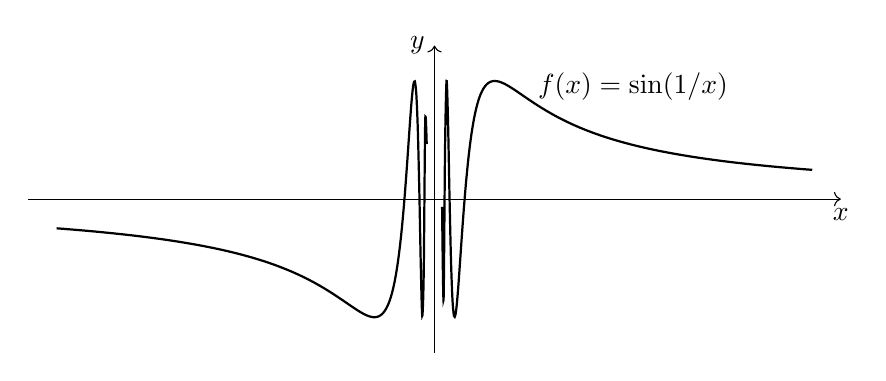
\begin{tikzpicture}[x=1.2cm,y=1.5cm]
\draw[->] (-4.3,0) -- (4.3,0) node[below] {$x$};
\draw[->] (0,-1.3) -- (0,1.3) node[left] {$y$};
\draw[thick,smooth,domain=-4:-0.08,samples=250] plot (\x,{sin(deg(1/\x))});
\draw[thick,smooth,domain=0.08:4,samples=250] plot (\x,{sin(deg(1/\x))});
\draw[dashed] (0,-1.05) -- (0,1.05);
\draw (2.1,0.95) node {$f(x)=\sin(1/x)$};
\end{tikzpicture}
\end{center}

\section*{3. 中間値の定理}

\begin{theorem}
$f$ を閉区間 $[a,b]$ で連続な関数とする。
\begin{itemize}
\item $f(a)\le f(b)$ なら，任意の $\lambda \in [f(a),f(b)]$ に対し，ある $c \in [a,b]$ があって $f(c)=\lambda$。
\item $f(a)\ge f(b)$ なら，任意の $\lambda \in [f(b),f(a)]$ に対し，ある $c \in [a,b]$ があって $f(c)=\lambda$。
\end{itemize}
\end{theorem}

\begin{center}
\begin{minipage}[t]{0.45\linewidth}
\centering
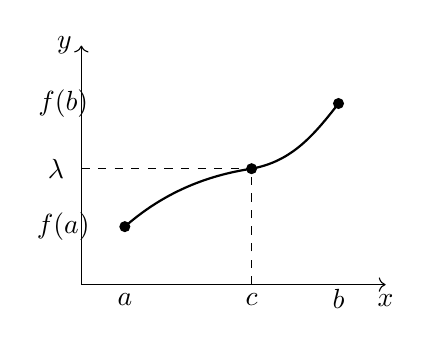
\begin{tikzpicture}[x=0.92cm,y=0.92cm]
\draw[->] (0,0) -- (4.2,0) node[below] {$x$};
\draw[->] (0,0) -- (0,3.3) node[left] {$y$};
\draw[thick] (0.6,0.8)
  .. controls (1.0,1.15) and (1.55,1.48) .. (2.35,1.6)
  .. controls (2.9,1.7) and (3.2,2.05) .. (3.55,2.5);
\draw[dashed] (0,1.6) -- (2.35,1.6);
\draw[dashed] (2.35,0) -- (2.35,1.6);
\fill (0.6,0.8) circle (2pt);
\fill (3.55,2.5) circle (2pt);
\fill (2.35,1.6) circle (2pt);
\draw (0.6,-0.2) node {$a$};
\draw (3.55,-0.2) node {$b$};
\draw (2.35,-0.2) node {$c$};
\draw (-0.25,0.8) node {$f(a)$};
\draw (-0.25,2.5) node {$f(b)$};
\draw (-0.35,1.6) node {$\lambda$};
\end{tikzpicture}

$f(a)\le f(b)$ の場合
\end{minipage}
\hfill
\begin{minipage}[t]{0.45\linewidth}
\centering
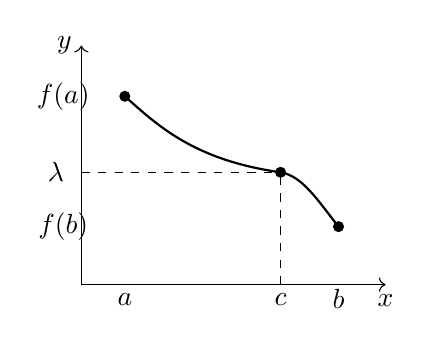
\begin{tikzpicture}[x=0.92cm,y=0.92cm]
\draw[->] (0,0) -- (4.2,0) node[below] {$x$};
\draw[->] (0,0) -- (0,3.3) node[left] {$y$};
\draw[thick] (0.6,2.6)
  .. controls (1.05,2.2) and (1.55,1.72) .. (2.75,1.55)
  .. controls (3.05,1.5) and (3.25,1.18) .. (3.55,0.8);
\draw[dashed] (0,1.55) -- (2.75,1.55);
\draw[dashed] (2.75,0) -- (2.75,1.55);
\fill (0.6,2.6) circle (2pt);
\fill (3.55,0.8) circle (2pt);
\fill (2.75,1.55) circle (2pt);
\draw (0.6,-0.2) node {$a$};
\draw (3.55,-0.2) node {$b$};
\draw (2.75,-0.2) node {$c$};
\draw (-0.25,2.6) node {$f(a)$};
\draw (-0.25,0.8) node {$f(b)$};
\draw (-0.35,1.55) node {$\lambda$};
\end{tikzpicture}

$f(a)\ge f(b)$ の場合
\end{minipage}
\end{center}

\section*{4. 微分の定義}

\begin{definition}
関数 $f$ が点 $a$ で微分可能であるとは，極限
\[
f'(a)=\lim_{h\to 0}\frac{f(a+h)-f(a)}{h}
\]
が存在することをいう。
\end{definition}

\begin{definition}
$f$ が区間 $I$ で微分可能であるとは，$I$ の各内点で微分可能であることをいう。
\end{definition}

微分可能ならば連続である。

\section*{5. 微分法則}

$f,g$ を区間 $I$ で微分可能な関数とする。

\begin{theorem}
\[
(f+g)'=f'+g',\qquad (fg)'=f'g+fg'
\]
\[
\left(\frac{f}{g}\right)'=\frac{f'g-fg'}{g^2}\qquad (g\ne 0)
\]
\[
(g\circ f)'(x)=g'(f(x))f'(x)
\]
\[
\frac{d}{dx}\log f(x)=\frac{f'(x)}{f(x)}\qquad (f(x)>0)
\]
\[
f'(x)=(\log f(x))'f(x)\qquad (f(x)>0)
\]
\end{theorem}

\subsection*{加法性の証明}

\begin{proof}
$a\in I$ とする。差商を計算すると
\[
\frac{(f+g)(a+h)-(f+g)(a)}{h}
=\frac{f(a+h)-f(a)}{h}+\frac{g(a+h)-g(a)}{h}
\]
である。$h\to 0$ とすると右辺は $f'(a)+g'(a)$ に収束するので，
\[
(f+g)'(a)=f'(a)+g'(a)
\]
を得る。
\end{proof}

\subsection*{対数微分の形}

たとえば
\[
f(x)=u(x)^{v(x)} \qquad (u(x)>0)
\]
ならば
\[
\log f(x)=v(x)\log u(x)
\]
より
\[
\frac{f'(x)}{f(x)}=v'(x)\log u(x)+v(x)\frac{u'(x)}{u(x)}
\]
したがって
\[
f'(x)=u(x)^{v(x)}\left(v'(x)\log u(x)+v(x)\frac{u'(x)}{u(x)}\right)
\]
である。

\ifPDFTeX
\end{CJK}
\fi

\end{document}
